
\documentclass[a4paper,11pt]{article}
\usepackage[a4paper, margin=8em]{geometry}

% usa i pacchetti per la scrittura in italiano
\usepackage[french,italian]{babel}
\usepackage[T1]{fontenc}
\usepackage[utf8]{inputenc}
\frenchspacing 

% usa i pacchetti per la formattazione matematica
\usepackage{amsmath, amssymb, amsthm, amsfonts}

% usa altri pacchetti
\usepackage{gensymb}
\usepackage{hyperref}
\usepackage{standalone}

% imposta il titolo
\title{Appunti Elettronica Digitale}
\author{Luca Seggiani}
\date{2026}

% imposta lo stile
% usa helvetica
\usepackage[scaled]{helvet}
% usa palatino
\usepackage{palatino}
% usa un font monospazio guardabile
\usepackage{lmodern}

\renewcommand{\rmdefault}{ppl}
\renewcommand{\sfdefault}{phv}
\renewcommand{\ttdefault}{lmtt}

% disponi il titolo
\makeatletter
\renewcommand{\maketitle} {
	\begin{center} 
		\begin{minipage}[t]{.8\textwidth}
			\textsf{\huge\bfseries \@title} 
		\end{minipage}%
		\begin{minipage}[t]{.2\textwidth}
			\raggedleft \vspace{-1.65em}
			\textsf{\small \@author} \vfill
			\textsf{\small \@date}
		\end{minipage}
		\par
	\end{center}

	\thispagestyle{empty}
	\pagestyle{fancy}
}
\makeatother

% disponi teoremi
\usepackage{tcolorbox}
\newtcolorbox[auto counter, number within=section]{theorem}[2][]{%
	colback=blue!10, 
	colframe=blue!40!black, 
	sharp corners=northwest,
	fonttitle=\sffamily\bfseries, 
	title=~\thetcbcounter: #2, 
	#1
}

% disponi definizioni
\newtcolorbox[auto counter, number within=section]{definition}[2][]{%
	colback=red!10,
	colframe=red!40!black,
	sharp corners=northwest,
	fonttitle=\sffamily\bfseries,
	title=~\thetcbcounter: #2,
	#1
}

% U.D.M
\newcommand{\amp}{\ensuremath{\mathrm{A}}}
\newcommand{\volt}{\ensuremath{\mathrm{V}}}
\newcommand{\meter}{\ensuremath{\mathrm{m}}}
\newcommand{\second}{\ensuremath{\mathrm{s}}}
\newcommand{\farad}{\ensuremath{\mathrm{F}}}
\newcommand{\henry}{\ensuremath{\mathrm{H}}}
\newcommand{\siemens}{\ensuremath{\mathrm{S}}}

% circuiti
\usepackage{circuitikz}
\usetikzlibrary{babel}

% disegni
\usepackage{pgfplots}
\pgfplotsset{width=10cm,compat=1.9}

% disponi codice
\usepackage{listings}
\usepackage[table]{xcolor}

\definecolor{codegreen}{rgb}{0,0.6,0}
\definecolor{codegray}{rgb}{0.5,0.5,0.5}
\definecolor{codepurple}{rgb}{0.58,0,0.82}
\definecolor{backcolour}{rgb}{0.95,0.95,0.92}

\lstdefinestyle{codestyle}{
		backgroundcolor=\color{black!5}, 
		commentstyle=\color{codegreen},
		keywordstyle=\bfseries\color{magenta},
		numberstyle=\sffamily\tiny\color{black!60},
		stringstyle=\color{green!50!black},
		basicstyle=\ttfamily\footnotesize,
		breakatwhitespace=false,         
		breaklines=true,                 
		captionpos=b,                    
		keepspaces=true,                 
		numbers=left,                    
		numbersep=5pt,                  
		showspaces=false,                
		showstringspaces=false,
		showtabs=false,                  
		tabsize=2
}

\lstdefinestyle{shellstyle}{
		backgroundcolor=\color{black!5}, 
		basicstyle=\ttfamily\footnotesize\color{black}, 
		commentstyle=\color{black}, 
		keywordstyle=\color{black},
		numberstyle=\color{black!5},
		stringstyle=\color{black}, 
		showspaces=false,
		showstringspaces=false, 
		showtabs=false, 
		tabsize=2, 
		numbers=none, 
		breaklines=true
}

\lstdefinelanguage{javascript}{
	keywords={typeof, new, true, false, catch, function, return, null, catch, switch, var, if, in, while, do, else, case, break},
	keywordstyle=\color{blue}\bfseries,
	ndkeywords={class, export, boolean, throw, implements, import, this},
	ndkeywordstyle=\color{darkgray}\bfseries,
	identifierstyle=\color{black},
	sensitive=false,
	comment=[l]{//},
	morecomment=[s]{/*}{*/},
	commentstyle=\color{purple}\ttfamily,
	stringstyle=\color{red}\ttfamily,
	morestring=[b]',
	morestring=[b]"
}

% disponi sezioni
\usepackage{titlesec}

\titleformat{\section}
	{\sffamily\Large\bfseries} 
	{\thesection}{1em}{} 
\titleformat{\subsection}
	{\sffamily\large\bfseries}   
	{\thesubsection}{1em}{} 
\titleformat{\subsubsection}
	{\sffamily\normalsize\bfseries} 
	{\thesubsubsection}{1em}{}

% disponi alberi
\usepackage{forest}

\forestset{
	rectstyle/.style={
		for tree={rectangle,draw,font=\large\sffamily}
	},
	roundstyle/.style={
		for tree={circle,draw,font=\large}
	}
}

% disponi algoritmi
\usepackage{algorithm}
\usepackage{algorithmic}
\makeatletter
\renewcommand{\ALG@name}{Algoritmo}
\makeatother

% disponi numeri di pagina
\usepackage{fancyhdr}
\fancyhf{} 
\fancyfoot[L]{\sffamily{\thepage}}

\makeatletter
\fancyhead[L]{\raisebox{1ex}[0pt][0pt]{\sffamily{\@title \ \@date}}} 
\fancyhead[R]{\raisebox{1ex}[0pt][0pt]{\sffamily{\@author}}}
\makeatother

\begin{document}
% sezione (data)
\section{Lezione del 04-05-26}

% stili pagina
\thispagestyle{empty}
\pagestyle{fancy}

% testo
Nella scorsa lezione abbiamo visto i regolatori di tensione in modalità \textit{switching}, in particolare nella configurazione "forward". Vediamo che esiste un ulteriore configurazione, che denominiamo "flyback".

\subsubsection{Flyback}
Nel \textbf{regolatore switching "flyback"} si ha la stessa topologia del regolatore in swtiching di tipo \textit{forward}, ma con l diodo e l'induttore scambiati fra di loro.

\begin{center}
\begin{tikzpicture}[transform shape]
	% Paths, nodes and wires:
	\draw (3, 5) to[battery1, l={$E$}] (3, 3);
	\draw (3, 5) to[switch] (5, 5);
	\draw (5, 5) to[cute inductor, l={$L$}] (5, 3);
	\draw (3, 3) -- (5, 3);
	\draw (5, 5) -- (6, 5);
	\draw (8, 5) to[empty diode, l={$D$}] (6, 5);
	\draw (8, 5) to[capacitor, l={$C$}] (8, 3);
	\draw (10, 5) to[american resistor, l={$R$}] (10, 3);
	\draw (8, 3) |- (5, 3);
	\draw (8, 3) -- (10, 3);
	\draw (8, 5) -- (10, 5);
\end{tikzpicture}
\end{center}

Vediamo il funzionamento di questa configurazione. Qui abbiamo due casi principali:
\begin{itemize}
	\item $T_{on}$, $D_{off}$: se alziamo la tensione a sinistra di $D$ (chiudendo l'interruttore) abbiamo che il diodo va in interdizione. In questo caso il generatore carica solamente l'induttanza, mentre la tensione alla resistenza $R$ viene mantenuta dalla capacità $C$ (con polarità opposta rispetto al forward, cioè con il $+$ in basso della $R$);
	\item $T_{off}$, $D_{on}$: quando l'interruttore si apre, il diodo va in conduzione, e l'induttanza può caricare la capacità (perché mantenga tensione stabile a $R$ al prossimo ciclo). 
\end{itemize}

Abbiamo quindi ottenuto una configurazione dove il generatore di tensione $E$ non è mai collegato direttamente al carico $R$, e quindi la polarità risulta invertita.

Anche in questo caso può essere utile considerare la caduta di tensione sull'induttanza.
\begin{itemize}
	\item Questa, quando l'interruttore è chiuso, sarà fissa ad $E$;
	\item Quando l'interruttore è aperto, invece, questa va a $-{V}_u$, cioè la tensione imposta su $R$.
\end{itemize}

Come per il caso forward, la tensione media sull'induttanza sarà nulla sul periodo $T_S$, per cui dovrà essere che:
$$
E T_{on} = V_u T_{off}
$$
e visto che $T_{off} = T_S - T_{on}$ si ha che:
$$
E T_{on} = V_u T_S - V_u T_{on} \implies E = V_u \left( \frac{1 - D}{D} \right) \implies V_u = E \frac{D}{1 - D}
$$
cioè una relazione diversa rispetto a quella del forward.

Abbiamo quindi la particolarità del flyback, cioè che il guadagno può essere maggiore di $1$:
$$
\frac{D}{1 - D} > 1 \implies D > \frac{1}{2}
$$
semplicemente ponendo duty cycle maggiore di $\frac{1}{2}$. Questo rende il flyback molto vantaggioso, e per questo motivo risulta ampiamente impiegato in elettronica.

\subsection{Stage di power supply}
Abbiamo quindi visto tutti i componenti che solitamente formano una \textit{power supply}, cioè un'unità di alimentazione per componenti elettronici. Questi sono:
\begin{itemize}
	\item Il \textit{ponte di Graetz}, che fa da \textbf{rettificatore} (porta la AC in DC);
	\item Il \textit{filtro RC}, che fa da \textbf{filtro} (e permette quindi di eliminare effetti di \textit{ripple} o comunque discontinuità dell'onda generata);
	\item Il \textit{regolatore di tensione}, che può essere di tipo switching o flyback, che ha il compito di stabilizzare la tensione filtrata ad un valore di riferimento.
\end{itemize}

Configuriamo tali componenti come segue per realizzare un alimentatore:
\begin{center}
\begin{tikzpicture}[transform shape]
	% Paths, nodes and wires:
	\node[shape=rectangle, draw, line width=1pt, minimum width=1.965cm, minimum height=1.965cm] at (4, 5){} node[anchor=center, align=center, text width=1.577cm, inner sep=6pt] at (4, 5){\footnotesize Ponte di\\Graetz};
	\draw (1, 4.5) -- (3, 4.5) -| (3, 5.5) -- (1, 5.5);
	\draw (5, 4.5) -- (6, 4.5) -| (6, 5.5) -- (5, 5.5) -| (5, 4.5);
	\node[shape=rectangle, draw, line width=1pt, minimum width=1.965cm, minimum height=1.965cm] at (7, 5){} node[anchor=center, align=center, text width=1.577cm, inner sep=6pt] at (7, 5){\footnotesize Filtro RC};
	\draw (8, 4.5) -- (9, 4.5) -| (9, 5.5) -- (8, 5.5) -| (8, 4.5);
	\node[shape=rectangle, draw, line width=1pt, minimum width=1.965cm, minimum height=1.965cm] at (10, 5){} node[anchor=center, align=center, text width=1.577cm, inner sep=6pt] at (10, 5){\footnotesize Regolatore di tensione};
	\draw (13, 5.5) -- (11, 5.5) -| (11, 4.5) -- (13, 4.5);
	\draw (13, 5.5) to[american resistor, /tikz/circuitikz/bipoles/length=0.700cm, v^=$V_u$, voltage=american] (13, 4.5);
	\draw (1, 5.5) to[american voltage source, /tikz/circuitikz/bipoles/length=0.700cm, l_={$220 \, \mathrm{V} / 50 \, \mathrm{Hz}$}] (1, 4.5);
\end{tikzpicture}
\end{center}

Abbiamo però che questa configurazione non rispetta le normative di sicurezza, in quanto esiste un percorso che va dalla tensione a $220 \, \mathrm{V}$. Per questo motivo solitamente si pone alla fine della catena un elemento di \textit{isolamento galvanico}, che può essere:
\begin{itemize}
	\item Un \textit{condensatore}, che imposto un voltaggio alle due armature ffettivamente blocca il passaggio della corrente;
	\item Un elemento di isolamento \textit{ottico}, che si basa su segnali luminosi per trasferire tensione;
	\item Come molto più tipico, un \textit{trasformatore}.
\end{itemize}

Per spiegarci come mai abbiamo bisogno di isolamento, vediamo uno schema che modellizza una qualsiasi apparecchiatura elettronica collegata alla rete elettrica:
\begin{center}
\begin{tikzpicture}[transform shape]
	% Paths, nodes and wires:
	\node[shape=rectangle, draw, line width=1pt, minimum width=2.215cm, minimum height=2.215cm] at (1.375, 1.125){};
	\draw (-1.75, 0.5) -| (0.25, 1.5) -- (-1.75, 1.5);
	\node[ground] at (-1.75, 0.5){};
	\node[shape=rectangle, minimum width=0.965cm, minimum height=0.465cm] at (-1.75, 1.75){} node[anchor=center, align=center, text width=0.577cm, inner sep=6pt] at (-1.75, 1.75){$220 \, \mathrm{V} / 50 \, \mathrm{Hz}$};
	\draw (0.75, 0.5) to[american resistor, /tikz/circuitikz/bipoles/length=0.700cm, l={$Z_2$}] (1.75, 0.5);
	\draw (1.75, 0.5) -| (1.75, 1.5);
	\draw (0.75, 1.5) to[american resistor, /tikz/circuitikz/bipoles/length=0.700cm, l={$Z_1$}] (1.75, 1.5);
	\draw (0.75, 1.5) -- (0.25, 1.5);
	\draw (0.25, 0.5) -- (0.75, 0.5);
\end{tikzpicture}
\end{center}

Abbiamo che questa offre un'impedenza $Z_1$ alla fase dalla cabina di distribuzione (che si trova a $220 \, \mathrm{V}$ RMS, $50 \, \mathrm{Hz}$), e un'altra impedenza $Z_2$ al neutro, che solitamente è a riferimento a $0 \, \mathrm{V}$. Toccando accidentalmente una parte del circuito che è oltre l'impedenza $Z_2$, l'operatore umano si troverebbe a toccare un punto potenzialmente a centinaia di volts, cosa chiaramente poco salutare al corpo umano. La soluzione adottata è quindi quella di munirsi di un trasformatore:
\begin{center}
\begin{tikzpicture}[transform shape]
	% Paths, nodes and wires:
	\node[shape=rectangle, draw, line width=1pt, minimum width=2.715cm, minimum height=2.215cm] at (1.625, 1.125){};
	\draw (-1.75, 0.5) -| (0.25, 1.5) -- (-1.75, 1.5);
	\node[ground] at (-1.75, 0.5){};
	\node[shape=rectangle, minimum width=0.965cm, minimum height=0.465cm] at (-1.75, 1.75){} node[anchor=center, align=center, text width=0.577cm, inner sep=6pt] at (-1.75, 1.75){$220 \, \mathrm{V} / 50 \, \mathrm{Hz}$};
	\draw (1.748, 0.5) to[american resistor, /tikz/circuitikz/bipoles/length=0.700cm, l={$Z_2$}] (2.747, 0.5);
	\draw (2.747, 0.5) -| (2.747, 1.5);
	\draw (1.748, 1.5) to[american resistor, /tikz/circuitikz/bipoles/length=0.700cm, l={$Z_1$}] (2.747, 1.5);
	\draw (1.748, 1.5) -- (1.247, 1.5);
	\draw (1.247, 0.5) -- (1.748, 0.5);
	\node[transformer, cute, xscale=0.475, yscale=0.475] at (0.749, 0.999){};
\end{tikzpicture}
\end{center}

In questo caso il circuito a destra si trova flottante rispetto ai $220 \, \mathrm{V}$, per cui toccando un qualsiasi punto non viene imposta alcuna corrente attraverso il corpo umano. Questo chiaramente finché si tocca un solo punto del circuito: più punti possono comunque trovarsi a tensioni diverse, per cui si potrebbe comunque incorrere nella folgorazione.

La problematica di questo approccio è data dal fatto che è difficile avere trasformatori che lavorino bene a $50 \, \mathrm{Hz}$, in dimensioni e pesi contenuti. Di contro, è piuttosto realizzare trasformatori a bassa tensione che funzionino a frequenze molto più elevate. Queste sono le frequenze a cui lavorano i regolatori switching, motivo per cui li troviamo molto più semplici da utilizzare per realizzare alimentatori. 

La configurazione è quindi la seguente:
\begin{center}
\begin{tikzpicture}[scale = 0.7, transform shape]
	% Paths, nodes and wires:
	\draw (-3, 2) -- (-1, 2);
	\draw (-3, -0) -- (-1, -0);
	\node[shape=rectangle, draw, line width=1pt, minimum width=1.965cm, minimum height=1.965cm] at (0, 1){} node[anchor=center, align=center, text width=1.577cm, inner sep=6pt] at (0, 1){Ponte di Graetz};
	\draw (1, -0) -- (2, -0);
	\draw (1, 2) -- (2, 2);
	\draw (2, 2) to[capacitor, l={$C1$}] (2, -0);
	\draw (2, 2) to[switch] (5, 2);
	\draw (2, -0) -- (5, -0);
	\node[transformer, cute, xscale=0.95, yscale=0.95] at (6.003, 1.003){};
	\draw (7, 0.005) -| (8, -0);
	\draw (7, 2) -- (8, 2);
	\draw (8, 2) to[empty diode, l={$D1$}] (10, 2);
	\draw (10, -0) to[empty diode, l={$D2$}] (10, 2);
	\draw (8, -0) -- (10, -0);
	\draw (10, 2) to[american inductor, l={$L$}] (12, 2);
	\draw (12, 2) to[capacitor, l={$C2$}] (12, -0);
	\draw (12, -0) |- (10, -0);
	\draw (14, 2) to[american resistor, l={$R$}] (14, -0);
	\draw (12, 2) -- (14, 2);
	\draw (12, -0) -- (14, -0);
	\draw (-3, 2) to[american voltage source, l_={$220 \, \mathrm{V} / 50 \, \mathrm{Hz}$}] (-3, -0);
\end{tikzpicture}
\end{center}

Dove abbiamo bisogno di 2 diodi anziché uno in quanto il trasformatore non pone il nodo al di sotto di $D2$ a 0 volts (e quindi dobbiamo bloccare la corrente). Questa configurazione permette quindi di impiegare un trasformatore, su una tensione che è sempre variabile in AC (si trova a valle del commutatore), ma che ha frequenza $>> 50 \, \mathrm{Hz}$ (sempre data dal commutatore e dalla sua logica di controllo), per cui gli ingombri e il peso del trasformatore risultano di molto ridotti (e si possono realizzare PSU di dimensioni ridotte). 

Vediamo quindi che il circuito completo è solitamente un circuito in \textit{retroazione}. Quello che abbiamo visto finora, infatti, è il componente della PSU in modalità switching detto \textit{DC-DC converter} (convertitore da continua a continua, a diverse tensioni). Per assicurarsci che la tensione in uscita sia costante avremo bisogno di un elemento di controllo, che altera la frequenza di commutazione dell'interruttore attraverso una certa logica di controllo:
\begin{center}
\begin{tikzpicture}[scale = 0.7, transform shape]
	% Paths, nodes and wires:
	\draw (-3, 2) -- (-1, 2);
	\draw (-3, -0) -- (-1, -0);
	\node[shape=rectangle, draw, line width=1pt, minimum width=1.965cm, minimum height=1.965cm] at (0, 1){} node[anchor=center, align=center, text width=1.577cm, inner sep=6pt] at (0, 1){Ponte di Graetz};
	\draw (1, -0) -- (2, -0);
	\draw (1, 2) -- (2, 2);
	\draw (2, 2) to[capacitor, l={$C1$}] (2, -0);
	\draw (2, 2) to[switch] (5, 2);
	\draw (2, -0) -- (3.36, -0);
	\node[transformer, cute, xscale=0.95, yscale=0.95] at (6.002, 1.003){};
	\draw (7, 0.005) -| (8, -0);
	\draw (7, 2) -- (8, 2);
	\draw (8, 2) to[empty diode, l={$D1$}] (10, 2);
	\draw (10, -0) to[empty diode, l={$D2$}] (10, 2);
	\draw (8, -0) -- (10, -0);
	\draw (10, 2) to[american inductor, l={$L$}] (12, 2);
	\draw (12, 2) to[capacitor, l={$C2$}] (12, -0);
	\draw (12, -0) |- (10, -0);
	\draw (14, 2) to[american resistor, l={$R$}] (14, -0);
	\draw (12, 2) -- (14, 2);
	\draw (12, -0) -- (14, -0);
	\draw (-3, 2) to[american voltage source, l_={$220 \, \mathrm{V} / 50 \, \mathrm{Hz}$}] (-3, -0);
	\draw (14, -0) |- (10, -1);
	\node[op amp, xscale=-1] at (8.81, -1.49){};
	\draw (10, -1.98) -| (11, -2) -| (11, -3);
	\node[shape=rectangle, minimum width=0.965cm, minimum height=0.715cm] at (11, -3.375){} node[anchor=center, align=center, text width=0.577cm, inner sep=6pt] at (11, -3.375){$V_{ref}$};
	\node[shape=rectangle, draw, line width=1pt, minimum width=1.965cm, minimum height=1.965cm] at (3.5, -1.5){} node[anchor=center, align=center, text width=1.577cm, inner sep=6pt] at (3.5, -1.5){Logica di controllo};
	\draw (7.62, -1.49) -| (4.5, -1.5);
	\node[jump crossing, rotate=-90] at (3.5, -0){};
	\draw (3.64, -0) -| (5.005, 0.005);
	\draw (3.5, -0.5) -- (3.5, -0.14);
	\draw (3.5, 1.75) -- (3.5, 0.14);
	\draw[dash pattern={on 0.4pt off 1.6pt}] (3.5, 1.75) -- (3.255, 2);
\end{tikzpicture}
\end{center}

\subsection{Segnali digitali}
Veniamo quindi alla parte del corso che tratta i \textbf{segnali digitali}. Questi in generale sono definiti come sequenze finite di numeri, rappresentati da \textit{simboli}, che nell'ambito elettronico vengono associati a varie \textit{tensioni} di riferimento. Solitamente nella logica comune si definisce una coppia di intervalli di tensioni:
$$
"0" \rightarrow V_L \in [ V_{LMIN}, V_{LMAX} ]
$$
$$
"1" \rightarrow V_H \in [ V_{HMIN}, V_{HMAX} ]
$$
dove $V_L$ è la tensione che rappresenta il simbolo $0$ e $V_H$ è la tensione che rappresenta il simbolo $1$. Trovato un modo per rappresentare lo $0$ e l'$1$, quindi, si può rappresentare qualsiasi sequenza finita di numeri in base 2. Notiamo che i due intervalli $[ V_{LMIN}, V_{LMAX} ]$ e $[ V_{HMIN}, V_{HMAX} ]$ dovranno per forza essere disgiunti (con un certo margine di errore), altirmenti non si avrebbe più modo di determinare un valore logico dall'altro.

\subsubsection{Componenti digitali}
I componenti del'elettronica digitale solitamente non vengono descritti in termini di curva di corrente in funzione della tensione, controllando la risposta di una \textit{tensione di uscita} $V_{out}$ rispetto ad una certa \textit{tensione di ingresso} $V_{in}$. Chiamiamo questa caratteristica anche \textbf{VTC} (\textit{Voltage Transfer Characteristic}). 

Un componente che potevamo descrivere in termini di trasferimento di voltaggio era già stato studiato in questi appunti a 11.1, cioè l'\textit{inverter} a carico resistivo. Questo ha simbolo:
\begin{center}
\begin{tikzpicture}[transform shape]
	% Paths, nodes and wires:
	\node[ieeestd not port] at (0.485, -0){};
\end{tikzpicture}
\end{center}

\par\smallskip

Inoltre, nelle caratteristiche di interesse agli informatici abbiamo che la caratteristica VTC è idealizzata, cioè si hanno discontinuità dove la tensione "salta" dal valore logico massimo a quello minimo.

\begin{center}
	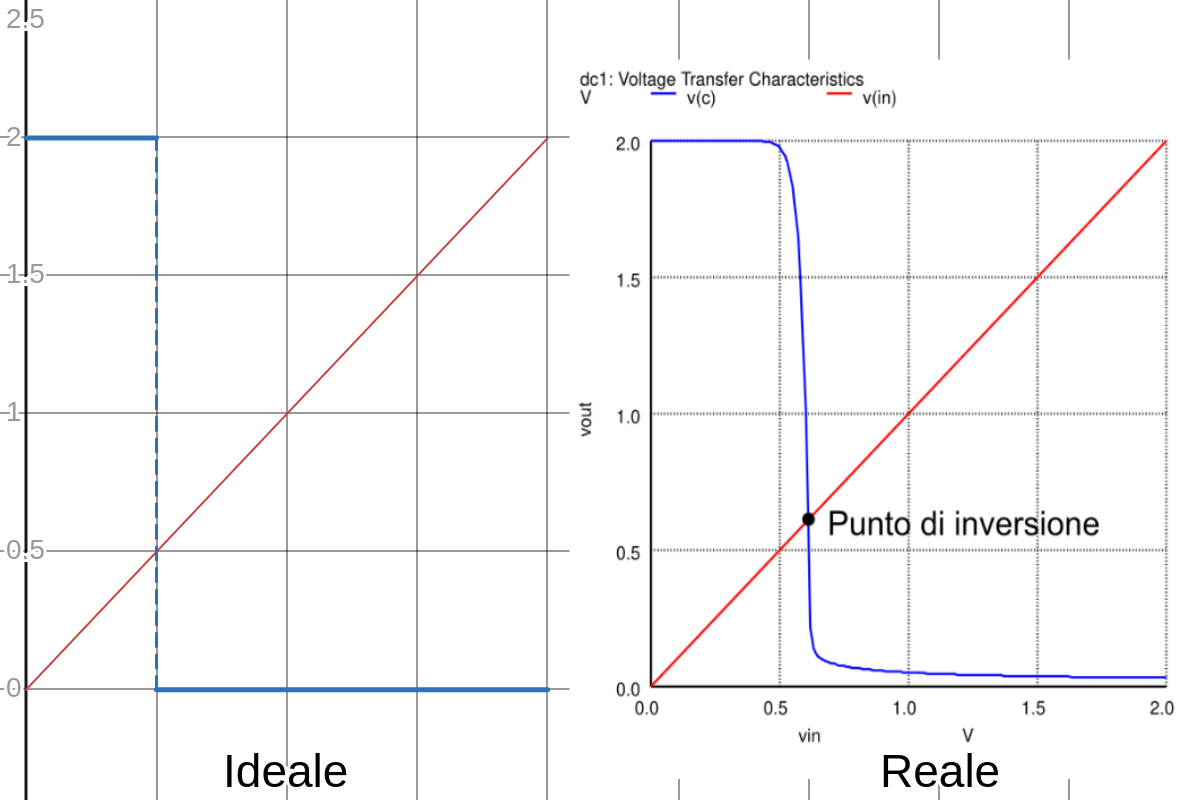
\includegraphics[scale=0.28]{../figures/real_ideal_digi.png}
\end{center}

Chiaramente questo è impossibile da realizzare nell'elettronica reale. Si decide quindi di scegliere i 2 punti sulla curva VTC che rispettano:
$$
\left| \frac{\partial V_{out}}{\partial V_{in}} \right| = 1
$$
e cioè dove la variazione di tensione in entrata e in uscita è identica (o alternativamente la pendenza della curva della VTC è $\pm 1$). 

\begin{center}
	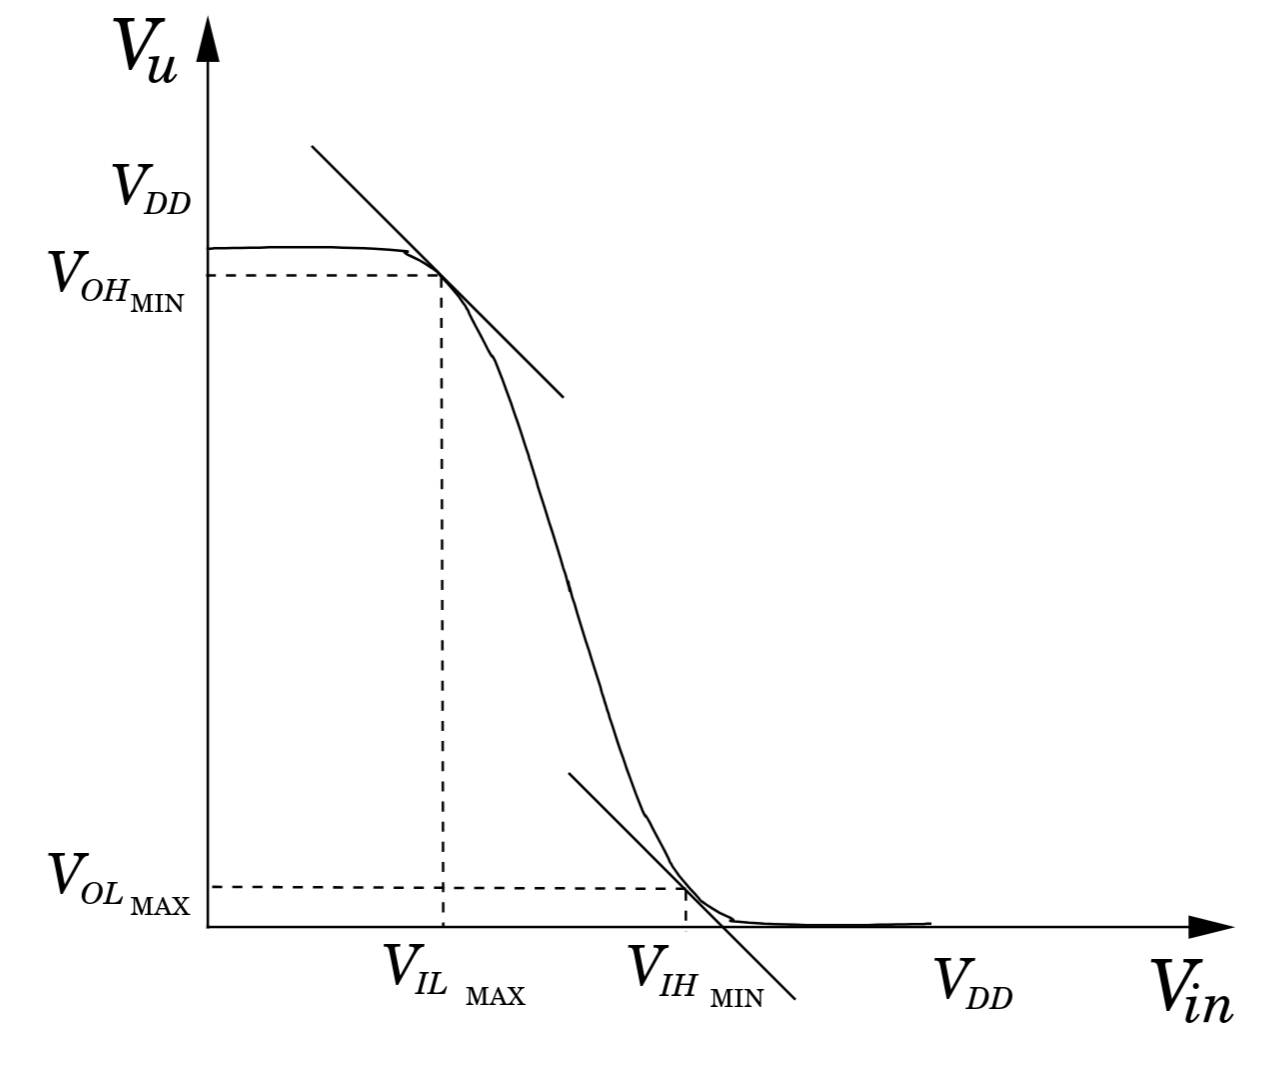
\includegraphics[scale=0.2]{../figures/vtc_points.png}
\end{center}

Nel caso (ad esempio) dell'inverter:
\begin{itemize}
\item Il punto che rispetta la condizione più prossimo al valore di uscita 1 (e quindi per l'inverter di entrata a 0) viene chiamato:
$$
( V_{IL MAX}, V_{OH MIN} )
$$
cioè individua la tensione di ingresso bassa massima per cui si ha il valore di uscita alto minimo;
\item Il punto che rispetta la condizione più prossimo al valore di uscita 0 (e quindi per l'inverter di entrata a 1) viene chiamato:
$$
( V_{IH MIN}, V_{OL MAX} )
$$
cioè individua la tensione di ingresso alta minima per cui si ha il valore di uscita basso massimo.
\end{itemize}
Viene da sé che tutta la regione da $V_{IL MAX}$ a $V_{IH MIN}$ è regione di \textit{transizione} dove il valore logico associato alla tensione di uscita o di ingresso non è ben specificato. 

\par\smallskip

\noindent
\textbf{\textsf{Margini di rumore}}

\noindent
Una problematica che ci interessa è data quando si mettono più di questi componenti in serie. 
\begin{center}
\begin{tikzpicture}[transform shape]
	% Paths, nodes and wires:
	\node[ieeestd not port](N1) at (0.485, -0){} node[anchor=center] at (N1.text){$1$};
	\node[ieeestd not port](N2) at (2.239, -0){} node[anchor=center] at (N2.text){$2$};
	\draw[-latex] (0.5, -2.25) -| (0.5, -1.5) -- (1, -1.5) -| (1, -0.5);
	\draw[-latex] (2, -2.25) -| (2, -1.5) -- (1.5, -1.5) -| (1.5, -0.5);
	\node[shape=rectangle, minimum width=1.6cm, minimum height=0.465cm] at (0.5, -2.5){} node[anchor=center, align=center, text width=1.4cm, inner sep=6pt] at (0.5, -2.5){\footnotesize Uscita 1};
	\node[shape=rectangle, minimum width=1.6cm, minimum height=0.465cm] at (2, -2.5){} node[anchor=center, align=center, text width=1.4cm, inner sep=6pt] at (2, -2.5){\footnotesize Entrata 2};
\end{tikzpicture}
\end{center}

Infatti, la nonlinearità dei componenti elettronici porta ad una distorsione dei valori logici in uscita dai componenti. Questo significa che andiamo a "mappare" i range di valori minimi e massimi in uscita, sui range di valori minimi e massima in entrata del componente in serie. Dovremmo quindi assicurare che la tensione in entrata al secondo componente (cioè in uscita dal primo) non vada a sforare le regioni valide per i valori logici.

\begin{center}
	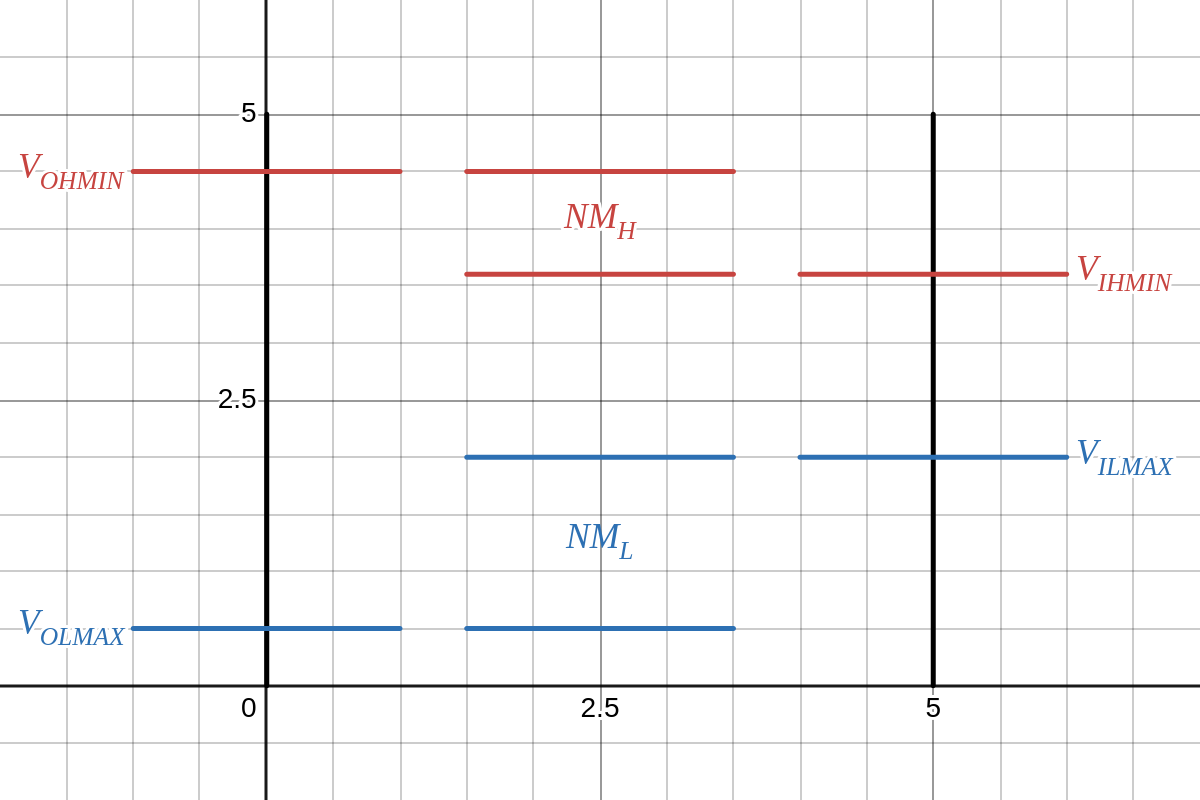
\includegraphics[scale=0.25]{../figures/noise_margins.png}
\end{center}

Definiamo quindi due parametri, detti \textit{margini di rumore}, che quantificano questa distorsione:
$$
N M_H = V_{OHMIN} - V_{IHMIN} > 0
$$
$$
N M_L = V_{ILMAX} - V_{OLMAX} > 0
$$
Quelli definiti sono rispettivamente i margini di rumore \textit{alto} e \textit{basso}, dove:
\begin{itemize}
	\item Il margine di rumore alto è dato dalla differenza fra il minimo valore logico considerato alto in uscita, e il minimo valore logico considerato alto in entrata;
	\item Il margine di rumore basso è dato dalla differenza fra il massimo valore logico considerato basso in entrata, e il massimo valore logico considerato alto in uscita;
\end{itemize}

\par\smallskip

\noindent
\textbf{\textsf{Porte rigenerative}}

\noindent
Una particolarità di alcune componentistiche digitali è il fatto che le porte sono \textit{rigenerative}. Questa è una caratteristica che permette al segnale di non degradarsi quando più porte vengono messe in cascata. Chiaramente, la rigenerazione delle porte richiede l'alimentazione dei componenti al $V_{cc}$ (cioè questi devono essere \textit{attivi}):
\begin{center}
\begin{tikzpicture}[transform shape]
	% Paths, nodes and wires:
	\node[ieeestd not port] at (0, -0){};
	\draw (0, 0.25) -| (0, 1);
	\draw (0, -0.25) -| (0, -1);
	\node[tlground] at (0, -1){};
	\node[vcc] at (0, 1){};
\end{tikzpicture}
\end{center}

Possiamo spiegarci come mai i componenti devono essere attivi guardando alla VTC.

\par\smallskip

\noindent
\textbf{\textsf{Considerazioni di potenza}}

\noindent
Possiamo fare delle considerazioni riguardo alla \textit{potenza dissipata} dai componenti digitali, cosa di fondamentale interesse per i dispositivi a risparmio energetico. Abbiamo che:
\begin{itemize}
	\item La potenza \textit{statica}, cioè quella consumata a vuoto dai componenti quando questi sono in equilibrio, è assolutamente da annullare (l'inverter a carico resistivo è pessimo in questo in quanto comporta un uso statico di potenza a fermo quando il valore logico di uscita è 1);
	\item La potenza \textit{dinamica}, cioè quella consumata per realizzare le transizioni di stato dei componenti (da alto a basso o viceversa) ci sarà sempre, ma vogliamo comunque minimizzarla.
\end{itemize}

\par\smallskip

\noindent
\textbf{\textsf{Considerazioni di temporizzazione}}

\noindent
Un'ulteriore caratteristica che vogliamo approfondire riguarda la \textit{temporizzazione} delle uscite dei componenti digitali rispetto agli ingressi.

Abbiamo diversi tempi caratteristici che vogliamo considerare. Innanzitutto rispetto alle transizioni stesse, abbiamo:
\begin{itemize}
	\item Il tempo $t_R$, detto \textit{rise time}, che rappresenta il tempo che l'entrata fisicamente impiega per arrivare dal valore logico minimo al valore logico massimo;
	\item Il tempo $t_F$, detto \textit{fall time}, che rappresenta il tempo che l'entrata fisicamente impiega per arrivare dal valore logico massimo al valore logico minimo;
\end{itemize}

Quini, per quanto riguarda la risposta a tali transizioni, definiamo:
\begin{itemize}
	\item Il tempo $t_{PHL}$, detto tempo di \textit{propagazione da alto a basso}, che rappresenta il tempo che il circuito impiega a rispondere ad una transizione abbassando la sua uscita;
	\item Il tempo $t_{PLH}$, detto tempo di \textit{propagazione da basso ad alto}, che rappresenta il tempo che il circuito impiega a rispondere ad una transizione alzando la sua uscita.
\end{itemize}

Da questi si definisce il tempo di \textit{ritardo medio} (o tempo di \textit{propagazione medio}):
$$
t_p = \frac{t_{PLH} + t_{PHL}}{2}
$$
Questo è un valore che non dipende dalla direzione delle transizioni, e per questo viene usato più spesso.

Infine notiamo il parametro:
$$
PDP = P_D \times t_p
$$
dove $P_D$ è la potenza dinamica impiegata e $t_p$ il tempo di propagazione medio. Questo valore rappresenta l'efficienza complessiva di un componente digitale, e a pari prestazioni preferiamo sicuramente il componente a $PDP$ minore (significa che ha $P_D$ potenza dissipata minore).

\par\smallskip

\noindent
\textbf{\textsf{Fan in / fan out}}

\noindent
Le ultime caratteristiche che vogliamo notare sono il \textit{fan in} e il \textit{fan out} del componente:
\begin{itemize}
	\item Il \textbf{fan in} è il numero massimo di ingressi che possiamo collegare alla porta;
	\item Il \textbf{fan out} è il numero massimo di uscite che possiamo collegare alla porta.
\end{itemize}

\end{document}
